\section{Acids, Bases and Salts} 

\begin{multicols}{2}


\section*{Acids and Bases} \index{Acids and bases}


\subsection{Acids in Daily Life}

\begin{center}
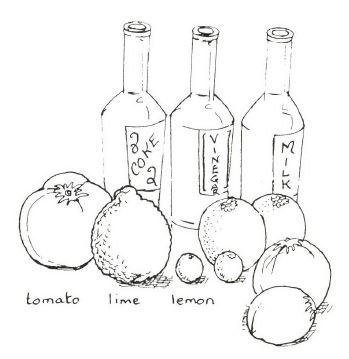
\includegraphics[width=0.4\textwidth]{./img/source/acids-daily.jpg}
\end{center}

\begin{description*}
%\item[Subtopic:]{}
%\item[Materials:]{}
%\item[Setup:]{}
\item[Procedure:]{Make a list of common acids seen in daily life.}
%\item[Hazards:]{}
%\item[Questions:]{}
\item[Observations:]{Citrus fruits (tomatoes, oranges, lemons etc.), vinegar, soda, sour milk and battery fluid are examples of everyday acids.}
%\item[Theory:]{}
%\item[Applications:]{}
%\item[Notes:]{}
\end{description*}

\subsection{Bases in Daily Life}

\begin{center}
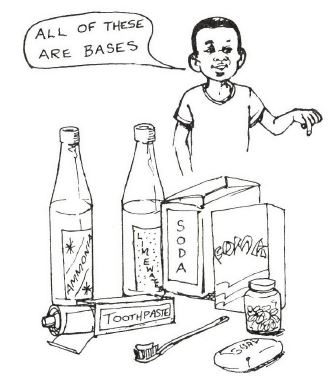
\includegraphics[width=0.4\textwidth]{./img/source/bases-daily.jpg}
\end{center}

\begin{description*}
%\item[Subtopic:]{}
%\item[Materials:]{}
%\item[Setup:]{}
\item[Procedure:]{Make a list of common acids seen in daily life.}
%\item[Hazards:]{}
%\item[Questions:]{}
\item[Observations:]{Soap, bicarbonate of soda, toothpaste, ammonia, limewater, cheese, fish, meat and indigestion tablets are all sources of bases.}
%\item[Theory:]{}
%\item[Applications:]{}
%\item[Notes:]{}
\end{description*}

\subsection{Acids React with Metals} \index{Metals! reaction with acids}

\begin{center}
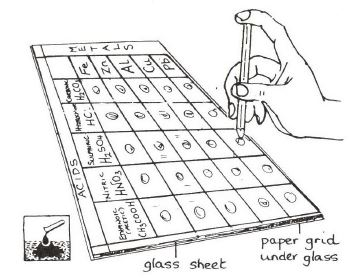
\includegraphics[width=0.4\textwidth]{./img/source/acid-metals.jpg}
\end{center}

\begin{description*}
%\item[Subtopic:]{}
\item[Materials:]{Syringe, sulphuric acid, zinc (from old dry cell)/nail/aluminium can}
%\item[Setup:]{}
\item[Procedure:]{Using a syringe, add a small amount of acid to various metals on a glass sheet.}
\item[Hazards:]{Do not use highly concentrated acids and wear goggles.}
%\item[Questions:]{}
\item[Observations:]{A gas is produced.}
\item[Theory:]{The gas produced is hydrogen, which can be confirmed with the `pop' test of holding a match nearby.}
%\item[Applications:]{}
%\item[Notes:]{}
\end{description*}

\subsection{Acids React with Carbonates}

\begin{center}
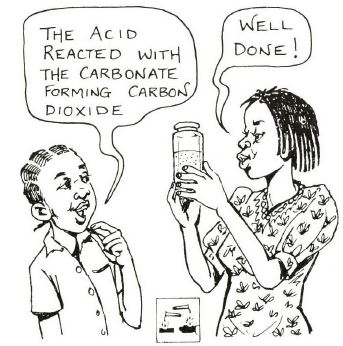
\includegraphics[width=0.4\textwidth]{./img/source/acids-bases.jpg}
\end{center}

\begin{description*}
%\item[Subtopic:]{}
\item[Materials:]{Bottle cap, dilute acid, baking powder, straw}
%\item[Setup:]{}
\item[Procedure:]{Add a few drops of dilute acid (e.g. vinegar, citric acid) to a bottle cap full of baking powder.}
%\item[Hazards:]{}
%\item[Questions:]{}
%\item[Observations:]{}
\item[Theory:]{Acid react with carbonates to form carbon dioxide.}
%\item[Applications:]{}
%\item[Notes:]{}
\end{description*}

\subsection{\textbf{CO}$_\textbf{2}$ Balloon} \index{Carbon dioxide! with acids and bases}

\begin{center}
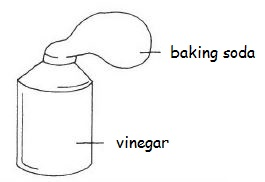
\includegraphics[width=0.2\textwidth]{./img/vso/co2-balloon.jpg}
\end{center}

\begin{description*}
%\item[Subtopic:]{}
\item[Materials:]{Bottle, baking soda, vinegar, balloon}
%\item[Setup:]{}
\item[Procedure:]{Add a small amount of vinegar into a bottle. Fill a balloon with baking soda (bicarbonate of soda) and stretch the balloon over the mouth of the bottle. Lift the balloon to empty the contents into the bottle.}
%\item[Hazards:]{}
%\item[Questions:]{}
\item[Observations:]{The balloon fills up with gas and may even explode!}
\item[Theory:]{The vinegar (acid) and baking soda (base) combine to produce carbon dioxide gas, which gets collected in the balloon.}
%\item[Applications:]{}
%\item[Notes:]{}
\end{description*}

\subsection{Making a Volcano} \index{Volcano} % PIC!!!

%\begin{center}
%\includegraphics[width=0.4\textwidth]{./img/.jpg}
%\end{center}

\begin{description*}
%\item[Subtopic:]{}
\item[Materials:]{Flour, sand, water, glue, vinegar, bicarbonate of soda, food colour}
\item[Setup:]{Create a model volcano (see \nameref{cha:models}, p.~\pageref{cha:models}). Add food colour if desired.}
\item[Procedure:]{Fill the pit of the volcano with bicarbonate of soda (with red food colour) and pour in the vinegar.}
%\item[Hazards:]{}
%\item[Questions:]{}
\item[Observations:]{A foamy `lava' erupts from the volcano.}
\item[Theory:]{Acids and bases react to produce a salt, carbon dioxide and water.}
\item[Applications:]{Use this as a science fair experiment at your school.}
%\item[Notes:]{}
\end{description*}

%\subsection{Acid Rain}
%
%\begin{center}
%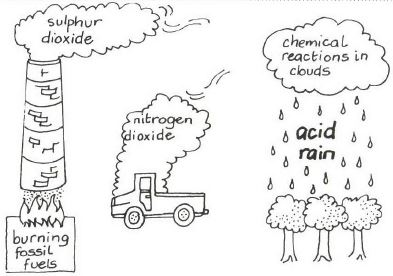
\includegraphics[width=0.4\textwidth]{./img/vso/acid-rain.jpg}
%\end{center}
%
%\begin{description*}
%%\item[Subtopic:]{}
%%\item[Materials:]{}
%%\item[Setup:]{}
%%\item[Procedure:]{}
%%\item[Hazards:]{}
%%\item[Questions:]{}
%%\item[Observations:]{}
%%\item[Theory:]{}
%\item[Applications:]{Pollution (e.g. from factories and cars) is carried in the wind and lowers the pH of the water droplets in the air. Eventually the water returns to the ground as acid rain, which may fall a long way from the cause of the pollution - often in a different country.}
%%\item[Notes:]{}
%\end{description*}

%\columnbreak

%==================================================================================================%

\section*{Indicators} 


\subsection{The pH Scale Line} \index{pH! scale}

\begin{center}
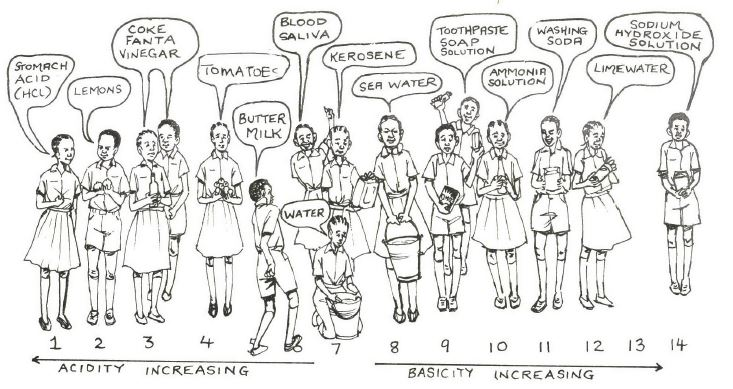
\includegraphics[width=0.49\textwidth]{./img/source/ph-line.jpg}
\end{center}

\begin{description*}
%\item[Subtopic:]{}
\item[Materials:]{Paper, various acids and bases shown}
%\item[Setup:]{}
\item[Procedure:]{Use chalk or string with paper numbers to mark out a pH scale in the classroom. Select some of the items shown and give one to each student. Ask
the student to stand at the correct place on the
scale.}
%\item[Hazards:]{}
%\item[Questions:]{}
%\item[Observations:]{}
%\item[Theory:]{}
%\item[Applications:]{}
%\item[Notes:]{}
\end{description*}

\columnbreak

\subsection{Making Indicators} \index{Indicators! preparation of}

\begin{center}
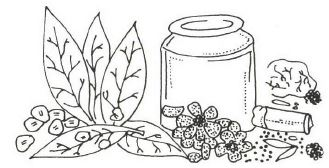
\includegraphics[width=0.4\textwidth]{./img/vso/making-indicators.jpg}
\end{center}

\begin{description*}
%\item[Subtopic:]{}
\item[Materials:]{Coloured flowers, fruits, leaves, water, \nameref{sec:heatsources}}
%\item[Setup:]{}
\item[Procedure:]{Gather different coloured flowers, fruits or leaves. Crush them up and add to boiled water or spirit.}
%\item[Hazards:]{}
%\item[Questions:]{}
%\item[Observations:]{}
\item[Theory:]{Many red, violet, yellow or pink flowers or fruits and leaves can be used
as indicators. Spirit-based indicators are more stable. Boiling improves the extraction
of colour. }
\item[Applications:]{Students could investigate which local flowers, leaves etc. produce the
most effective indicators.}
%\item[Notes:]{}
\end{description*}

\subsection{Testing for pH} % PIC!!!

%\begin{center}
%\includegraphics[width=0.4\textwidth]{./img/.jpg}
%\end{center}

\begin{description*}
%\item[Subtopic:]{}
\item[Materials:]{Rosella leaves, paper, straw, hot water, lemon or vinegar, bicarbonate of soda}
\item[Setup:]{Prepare an indicator solution from rosella leaves by crushing and adding to boiled water.}
\item[Procedure:]{Place a small amount of vinegar or lemon juice to one bottle cap and some bicarbonate of soda to another. Add a few drops of indicator to each cap, noting any colour changes that occur.}
%\item[Hazards:]{}
%\item[Questions:]{}
%\item[Observations:]{}
\item[Theory:]{The vinegar should turn a reddish colour, indicating it is acidic. The bicarbonate of soda a greenish or blue colour, indicating it is a basic.}
%\item[Applications:]{}
\item[Notes:]{Dip thin strips of paper in the indicator solution and let dry to make home-made litmus paper.}
\end{description*}

\columnbreak

\subsection{Exchanging Fluids}

\begin{center}
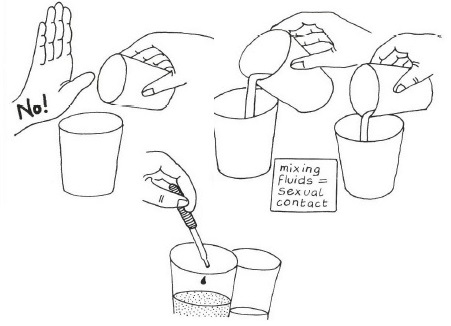
\includegraphics[width=0.49\textwidth]{./img/vso/hiv-passing.jpg}
\end{center}

\begin{description*}
%\item[Subtopic:]{}
\item[Materials:]{Plastic bottles, plastic bags, rubber bands or tape, phenolphthalein indicator, sodium hydroxide}
\item[Setup:]{Make a solution of NaOH (3-5 tablespoons in 500 mL water). The concentration should be enough so that multiple dilutions of the solution will still show a colour change when PoP is added. Cut enough plastic bottle cups so each student has one. Number each cup and separate into 3 groups (those who abstain, those who use condoms, and those who neither use condoms nor abstain). Make note of which numbers are in which group (but do not reveal until later). There should be at least 2 that abstain, 2 that use condoms, and the rest use neither. No more than 2 people total should start HIV positive (at least 1 being a sexually active non-condom user). Fill all the cups except the ones that will be HIV+ with about 100-200 mL of water. Fill the HIV+ cup(s) with the NaOH solution, making sure the volume is the same as the water-filled cups. Take the plastic bags (condoms) and secure them over each condom user's cup with tape or a rubber band. The plastic should have a slight dip so fluid can still be poured into it while preventing the fluids from mixing.}
\item[Procedure:]{Introduce the activity by stating that 1-2 of the cups is HIV+ but do not reveal which one(s). Announce which cup numbers will abstain (meaning which ones will not share fluids with anyone), which ones use condoms (meaning they can receive fluids but do not share them), and which ones use neither (meaning they will be exchanging fluids multiple times with multiple people). Show students that 1 of the non-condom users does not have HIV by adding 1-2 drops of PoP with no colour change. Then take a small sample of leftover NaOH solution and add 1 drop of PoP. Explain that a colour change to pink/purple, even very slight, means they are HIV+. Randomly give out the different cups and tell students to take 10-15 minutes to exchange fluids with others. Encourage them to return to other "partners" and exchange multiple times. (It is recommended that students mix fluids by pouring so enough fluid is transferred between the two cups.) After the time is up and enough exchanging of fluids has occurred, test every student's cup with 1-2 drops of PoP.}
\item[Hazards:]{Be careful when using concentrated NaOH. It can be very caustic if not handled with care. Neutralize spills with a weak acid (e.g. vinegar).}
\item[Questions:]{Which students ended up being HIV+ and why? How quickly did HIV spread?}
\item[Observations:]{If done correctly, every student except those who abstained or used condoms should test positive for HIV, as seen by a change in colour from the indicator.}
\item[Theory:]{Sodium hydroxide solution is a base, and bases turn pink/purple when PoP is added. Even though NaOH is colourless and difficult to tell apart from water (just as HIV+ people are difficult to tell apart from HIV- people), once it is present, it does not go away and can be spread very easily without protection. The activity also shows that even though there was only 1 or 2 people to start with HIV, it spread to practically every person who exchanged fluids (sexually active).}
\item[Applications:]{It is important to prevent oneself from getting HIV, and abstinence and using condoms are two highly effective methods of getting HIV.}
\item[Notes:]{Instead of using PoP indicator and a strong base, iodine can be used to test for starch. The same setup and procedure is followed, except the starch solution can be water from boiling potatoes, etc. Just make sure the starch solution and water are not distinguishable. 

Additionally, this activity can be used to explain the spread of malaria. Instead of every person exchanging fluids, there are 2 main groups: humans and female mosquitoes. This time, only students with syringes (female mosquitoes) inject their solution (saliva) into the human and suck the human's solution (blood) into their own cup. The sucking and injecting should again happen multiple times with multiple people. There can be different groups of humans (those who use mosquito nets, who do not get bit at all, etc.) and no more than 2 female mosquitoes should carry malaria to start.}
\end{description*}

\vfill
\columnbreak

%==================================================================================================%

\section*{Neutralisation} \index{Neutralisation}


\subsection{Neutralisation Reactions}

\begin{center}
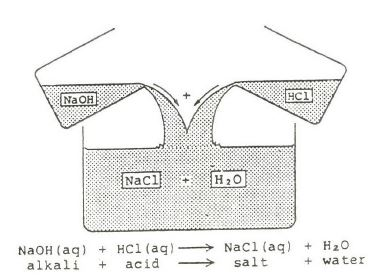
\includegraphics[width=0.49\textwidth]{./img/source/neutralisation.jpg}
\end{center}

\begin{description*}
%\item[Subtopic:]{}
\item[Materials:]{Sodium hydroxide solution, hydrochloric acid solution, bottles}
%\item[Setup:]{}
\item[Procedure:]{Prepare dilute solutions of sodium hydroxide and hydrochloric acid. Pour the two solutions together in a large container.}
\item[Hazards:]{Never use concentrated acids. Always wear goggles when using acids.}
%\item[Questions:]{}
%\item[Observations:]{}
\item[Theory:]{When acids and bases combine, they produce a salt and water. In this case the salt is sodium chloride. The resulting solution is neither acidic nor basic, but neutral.}
%\item[Applications:]{}
%\item[Notes:]{}
\end{description*}

\subsection{Ant Acid}

\begin{center}
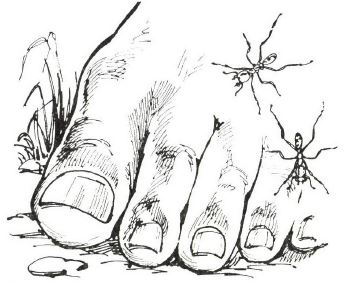
\includegraphics[width=0.4\textwidth]{./img/source/ant-acid.jpg}
\end{center}

\begin{description*}
%\item[Subtopic:]{}
%\item[Materials:]{}
%\item[Setup:]{}
%\item[Procedure:]{}
%\item[Hazards:]{}
%\item[Questions:]{}
%\item[Observations:]{}
%\item[Theory:]{}
\item[Applications:]{Many insects, such as bees and ants, inject an acidic liquid into the skin when they sting. The sting can be neutralized by rubbing baking soda (or other alkaline substances such as cucumber and avocado) on the affected area. Wasp stings, however, are alkaline and can be neutralized with vinegar (acetic acid).}
%\item[Notes:]{}
\end{description*}

\columnbreak

\subsection{Neutralisation in Daily Life}

\begin{center}
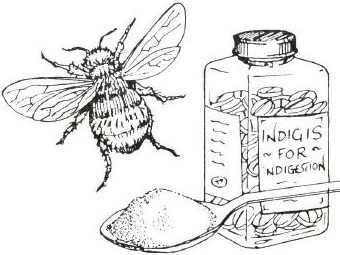
\includegraphics[width=0.3\textwidth]{./img/source/neutralisation-daily.jpg}
\end{center}

\begin{description*}
%\item[Subtopic:]{}
%\item[Materials:]{}
%\item[Setup:]{}
%\item[Procedure:]{}
%\item[Hazards:]{}
%\item[Questions:]{}
%\item[Observations:]{}
%\item[Theory:]{}
\item[Applications:]{Stomach aches are often caused by an excess of acid in the stomach. Taking antacids (magnesium or sodium bicarbonate) neutralizes the acid and relieves the pain. }
%\item[Notes:]{}
\end{description*}

%==================================================================================================%

\section*{Salts} \index{Salts}


\subsection{Preparation of Salts}

\begin{center}
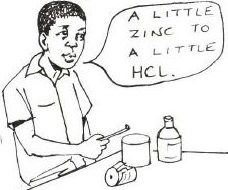
\includegraphics[width=0.25\textwidth]{./img/source/salt-acid-metal.jpg}
\end{center}

\begin{description*}
%\item[Subtopic:]{}
\item[Materials:]{Bottle cap, zinc (from dry cell), hydrochloric acid}
%\item[Setup:]{}
\item[Procedure:]{Add some zinc (found in dry cells) to hydrochloric acid.}
%\item[Hazards:]{}
%\item[Questions:]{}
%\item[Observations:]{}
\item[Theory:]{Acids and metals react to form salts. The chemical equation for this reaction is: \ce{Zn(s) + 2HCl $\longrightarrow$ ZnCl2(s) + H2(g)}}
%\item[Applications:]{}
%\item[Notes:]{}
\end{description*}

%\subsection{Preparation of Salts - Acid and Salt}
%
%\begin{center}
%\includegraphics[width=0.4\textwidth]{./img/.jpg}
%\end{center}
%
%\begin{description*}
%%\item[Subtopic:]{}
%\item[Materials:]{Bottle cap, limestone (calcium carbonate), hydrochloric acid}
%%\item[Setup:]{}
%\item[Procedure:]{To some pieces of limestone add a little hydrochloric acid.}
%%\item[Hazards:]{}
%%\item[Questions:]{}
%%\item[Observations:]{}
%\item[Theory:]{}
%\item[Applications:]{}
%\item[Notes:]{}
%\end{description*}

\subsection{Solubility of Salts}

\begin{center}
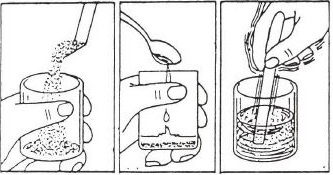
\includegraphics[width=0.35\textwidth]{./img/source/salt-solubility.jpg}
\end{center}

\begin{description*}
%\item[Subtopic:]{}
\item[Materials:]{Bottle caps, water, kitchen salt (sodium chloride), baking soda (sodium hydrogen carbonate), copper (II) sulphate, gypsum (calcium sulphate)}
%\item[Setup:]{}
\item[Procedure:]{For each salt: add a bottle cap full of salt to 5 caps of water and shake well. Observe which salts dissolve in water.}
%\item[Hazards:]{}
%\item[Questions:]{}
\item[Observations:]{All salts should dissolve except for gypsum (calcium sulphate).}
\item[Theory:]{Most sulphates, nitrates and chlorides are soluble in water, while most carbonates are not. Calcium sluphate and sodium carbonate are exceptions to these general rules.}
%\item[Applications:]{}
%\item[Notes:]{}
\end{description*}

%\subsection{Snow Globes}
%
%\begin{center}
%\includegraphics[width=0.4\textwidth]{./img/.jpg}
%\end{center}
%
%\begin{description*}
%%\item[Subtopic:]{}
%\item[Materials:]{}
%\item[Setup:]{}
%\item[Procedure:]{}
%\item[Hazards:]{}
%\item[Questions:]{}
%\item[Observations:]{}
%\item[Theory:]{}
%\item[Applications:]{}
%\item[Notes:]{}
%\end{description*}


\end{multicols}

\pagebreak